%; whizzy paragraph -pdf xpdf -latex ./whizzypdfptex.sh
%; whizzy-paragraph "^\\\\begin{frame}\\|\\\\emtext"
% latex beamer presentation.
% platex, latex-beamer でコンパイルすることを想定。 

%     Tokyo Debian Meeting resources
%     Copyright (C) 2012 Junichi Uekawa
%     Copyright (C) 2016 Nobuhiro Iwamatsu

%     This program is free software; you can redistribute it and/or modify
%     it under the terms of the GNU General Public License as published by
%     the Free Software Foundation; either version 2 of the License, or
%     (at your option) any later version.

%     This program is distributed in the hope that it will be useful,
%     but WITHOUT ANY WARRANTY; without even the implied warreanty of
%     MERCHANTABILITY or FITNESS FOR A PARTICULAR PURPOSE.  See the
%     GNU General Public License for more details.

%     You should have received a copy of the GNU General Public License
%     along with this program; if not, write to the Free Software
%     Foundation, Inc., 51 Franklin St, Fifth Floor, Boston, MA  02110-1301 USA

\documentclass[cjk,dvipdfmx,12pt]{beamer}
\usetheme{Tokyo}
\usepackage{monthlypresentation}

%  preview (shell-command (concat "evince " (replace-regexp-in-string "tex$" "pdf"(buffer-file-name)) "&")) 
%  presentation (shell-command (concat "xpdf -fullscreen " (replace-regexp-in-string "tex$" "pdf"(buffer-file-name)) "&"))
%  presentation (shell-command (concat "evince " (replace-regexp-in-string "tex$" "pdf"(buffer-file-name)) "&"))

%http://www.naney.org/diki/dk/hyperref.html
%日本語EUC系環境の時
\AtBeginDvi{\special{pdf:tounicode EUC-UCS2}}
%シフトJIS系環境の時
%\AtBeginDvi{\special{pdf:tounicode 90ms-RKSJ-UCS2}}

\newenvironment{commandlinesmall}%
{\VerbatimEnvironment
  \begin{Sbox}\begin{minipage}{1.0\hsize}\begin{fontsize}{8}{8} \begin{BVerbatim}}%
{\end{BVerbatim}\end{fontsize}\end{minipage}\end{Sbox}
  \setlength{\fboxsep}{8pt}
% start on a new paragraph

\vspace{6pt}% skip before
\fcolorbox{dancerdarkblue}{dancerlightblue}{\TheSbox}

\vspace{6pt}% skip after
}
%end of commandlinesmall

\title{Debian勉強会 / Debian JP Project}
\subtitle{OSC2016 北海道 出張版}
\author{岩松 信洋}
\date{2016年6月18日}
\logo{
\includegraphics[width=8cm]{image200607/openlogo-light.eps}}

\begin{document}

\begin{frame}
\titlepage{}
\end{frame}


\begin{frame}{ここにいる人たち}
\pause
\begin{itemize}[<+->]
\item 河田さん\\ 
	パッケージメンテナ  \pause
\item 倉敷さん \\ 
	Debian Developer になるべく修行中 \pause
\item 佐々木さん \\
	Ruby 使いのDebian Maintainer \pause
\item 吉野さん \\
	パッケージメンテナ。パッケージ翻訳マスター。\pause
\item 岩松 信洋 \\
	その辺にいるDebian Developer \pause
\end{itemize} 
\end{frame}

\begin{frame}{Agenda}
  \begin{itemize}
   \item Debian とは?
   \item Debian Updates
   \item Debian 9 情報
   \item 今後のイベント
  \end{itemize}
\end{frame}

\section{Debian とは?}
\begin{frame}\begin{center}\Huge{Debian とは?}\end{center}\end{frame}

\begin{frame}{Debian とは?}

{\color{red}{フリー/オープン}}な{\color{red}{ユニバーサル}}オペレーティングシステム を作成しようとするボランティアベースのプロジェクト。

\begin{table}[htb]
  \begin{tabular}{|c|c|c|}
    \hline
    ディストリ & 企業 & ボランティア \\ \hline
    RHEL & RedHat & なし  \\ \hline
    CentOS & RedHat & あり \\ \hline
    Ubuntu  & Canonical & あり \\ \hline
    \color{red}{Debian}  & \color{red}{なし} & \color{red}{あり} \\ \hline
  \end{tabular}
\end{table}

\end{frame}

\begin{frame}{Debian とは?}
Linux カーネルだけではなく、FreeBSD や GNU/Hurd のカーネルを利用したOSも提供。

% \begin{center}
% \includegraphics[width=0.3\hsize]{image201606/Freebsd-logo.jpg}
% \includegraphics[width=0.8\hsize]{image201606/hurd.png}
% \end{center}

\end{frame}

\begin{frame}{Debian とは?}

  \begin{itemize}
  \item Debian 社会契約(オープンソースの定義の元)
  \item Debian フリーソフトウェアガイドライン
  \item Debian Policy
  \end{itemize}

\end{frame}

\begin{frame}{Debian とは?}

\begin{minipage}{0.45\hsize}
  \begin{itemize}
\item Ubuntu や Raspbian といったディストリビューションのベースとなっている \\
	Debian Derivatives (Debian 派生ディストリビューション調査と協力体制の整備)
  \end{itemize}
\end{minipage} 
\begin{minipage}{0.45\hsize}
 \begin{center} 
 %   \includegraphics[width=1\hsize]{image201606/DebianFamilyTree1210.png}
 % https://en.wikipedia.org/wiki/List_of_Linux_distributions#/media/File:DebianFamilyTree1210.svg
 \end{center}
\end{minipage}

\end{frame}

\begin{frame}{Debian とは?}
 世界規模で開発が行われており、63ヶ国、約1000名のDebian公式開発者が開発を行
 っている。パッケージメンテナや翻訳などの貢献者も入れるともっと多くの開発者が参加
 していることになる。
% \begin{center}
%  \includegraphics[width=0.7\hsize]{image201606/group_photo_t.jpg}
% \end{center}
\end{frame}

\begin{frame}{Debian とは?}
\begin{itemize}[<+->]
 \item 2016年6月の時点で、\pause 最新版は Debian 8.5 (コードネーム Jessie)、\pause パッケージ数は約43000を提供、\pause
 公式にサポートするCPUアーキテクチャは10。\pause
 \item 約2年毎にリリース
 \begin{center}
 %\includegraphics[width=0.7\hsize]{image201605/i4282a1da3049189bccafa8929c4df0ab.png}
 \end{center}
 \item 次のリリース (コードネーム: Stretch)は 2018年Q2またはQ3の予定
 \item コードネームはトイ・ストーリのキャラクターを採用している。
%  \begin{center}
%  \includegraphics[width=0.5\hsize]{image201606/toy.jpg}
%  \end{center}
\end{itemize}
\end{frame}

\begin{frame}{Debian とは?}
どこで使われているのか?\pause
Linux ディストリビューションのベース

  \begin{center}
  % \includegraphics[width=0.5\hsize]{image201606/ubuntu.png}
  \end{center}

\end{frame}

\begin{frame}{Debian とは?}
Webサーバとして利用されてる(2016/06時点)

%  \begin{center}
%  \includegraphics[width=0.5\hsize]{image201606/w3techs.png}
%  \end{center}
  \tiny{\url{http://w3techs.com/technologies/details/os-linux/all/all}}

\end{frame}

\begin{frame}{Debian とは?}
組込デバイスのベースOSとして利用されている

% \begin{center}
% \includegraphics[width=0.5\hsize]{image201606/bbb-logo.jpeg}
 % http://www.tech-villa.com/images/kallyas_images/blog_images/beagleboneblack_logo.jpg
% \end{center}
 \url{http://beagleboard.org/}

% \begin{center}
% \includegraphics[width=0.2\hsize]{image201606/rpi-logo.png}
 % https://www.raspberrypi.org/wp-content/uploads/2015/08/raspberry-pi-logo.png
% \end{center}
 \url{https://www.raspberrypi.org/}

 \end{frame}

\begin{frame}{Debian とは?}

\begin{itemize}
\item ISS (国際宇宙ステーション)
\begin{center}
% \includegraphics[width=0.5\hsize]{image201606/STS-134_International_Space_Station_after_undocking}
% https://ja.wikipedia.org/wiki/%E5%9B%BD%E9%9A%9B%E5%AE%87%E5%AE%99%E3%82%B9%E3%83%86%E3%83%BC%E3%82%B7%E3%83%A7%E3%83%B3#/media/File:STS-134_International_Space_Station_after_undocking.jpg
\end{center}
{\tiny \url{https://training.linuxfoundation.org/why-our-linux-training/training-reviews/linux-foundation-training-prepares-the-international-space-station-for-linux-migration}}

\item Steam (ゲームPC OS)
\item NAS、ルータ
\item etc..
\end{itemize}

\end{frame}
\begin{frame}{Debian とは?}
まとめると\pause
\begin{itemize}[<+->]
\item Debianはフリー/オープンなオペレーティングシステム (OS)を作成しようとするボランティアベースのプロジェクト。
\item 自分たちの考えるフリーという言葉に関する定義、開発目的、パッケージングポリシーを厳格に決めている。
\item 世界中に1000人以上の開発者がおり、他のディストリビューションのベースとして採用されている。
\item 約2年毎にリリースが行われ、多くのパッケージとアーキテクチャをサポートしている。次期リリースは2018年Q2からQ3。
\item 上記のような特徴から様々なところで利用されているLinuxディストリビューションである。
\end{itemize}

\end{frame}

\begin{frame}{Debian JP Project とは?}
\pause
\begin{itemize}[<+->]
\item 日本でDebianを普及させることを目的とした任意団体。
\item Debian の日本語による情報発信、ユーザとの情報交換、Debian 開発者の育成など。
\end{itemize}
\end{frame}


\begin{frame}
\frametitle{Debian勉強会}
\begin{itemize}
 \item 2005年1月開始
 \item Debian Developer 上川さん発起人
\item 東京と関西で月に一回コンスタントに開催しているDebian開発者、ユーザによる勉強会。
\end{itemize}
\end{frame}

\begin{frame}

\frametitle{Debian勉強会:解決したい内容}
\begin{itemize}
 \item<1-> 問題
       \begin{itemize}
	\item MLとIRCで情報交換していた
	\item face-to-faceであう場所がない
	\item まとまったドキュメントが出てこない
       \end{itemize}
 \item<2-> Debian勉強会の提案
       \begin{itemize}
	\item 定期的に集まる
	\item 資料を必ず作成する。(GPLで!)
	  \ \ {\small \url{git://anonscm.debian.org/tokyodebian/monthly-report.git}}
       \end{itemize}
\end{itemize}

\end{frame}

\begin{frame}
 \frametitle{Debian勉強会:実際}
 \begin{itemize}
  \item Debian Weekly News Quiz
  \item Debian 界隈やパッケージング関連の話題など専門の人に話を聞く
  \item 前回の内容(東京):\\
	\begin{itemize}
	\item 場所: 朝日ネットさん
	\item Buffalo Linkstation向けDebian Installer 開発について
	\item Debian ハックタイム
	\end{itemize}
  \item 各地のイベントでDebian普及活動。 
	\begin{itemize}
	  \item 先月はOSC2016群馬に出展
	  \item 昨日はDebian/Ubuntu ユーザミートアップ in 札幌を開催
	\end{itemize}
 \end{itemize}
\end{frame}

\section{Debian Updates}
\begin{frame}\begin{center}\Huge{Debian Updates}\end{center}\end{frame}

\begin{frame}{Debian Updates}% [containsverbatim]

\begin{itemize}[<+->]
\item 2016/02/29: Debian 6 Long Term Support (LTS)終了\\
   \pause \small{LTSチームが利用企業からスポンサー支援を受け、i386, amd64, armelとarmhf
   のアーキテクチャに対してセキュリティアップデートを行う。\\
   期間は対象リリースのセキュリティサポートが切れてから約2年間。}
   \pause
\item 2016/04/02: Updated Debian 8: 8.4, Debian 7: 7.10
\item 2016/04/02: 2016年度 Debian Project Leader 決定\\
		今年度は Mehdi Dogguy 氏。OCaml や リリースチームメンバーとして活発に活動。
\end{itemize}

\end{frame}

\begin{frame}{Debian Updates}% [containsverbatim]

\begin{itemize}[<+->]
\item 2016/04/25: Debian 7.0(Wheezy) のセキュリティサポートが LTS チームに移行 \\
   \pause \small{Debian 7 は 2016年4月26日にサポートが切れたため、2018年5月31日までサポートされる。}

\item 2016/05/07: 次期リリース版である Debian 9のi386アーキテクチャのサポートCPUをi686以降に変更 

サポートが廃止されるx86プロセッサ
\begin{itemize}
\item Intel Pentium、Pentium with MMX
\item AMD K5、K6、K6-2 (aka K6 3D)、K6-3
\item VIA C3 Samuel 2、Ezra
\item IDT Winchip C6/2
\end{itemize}
{\tiny \url{https://lists.debian.org/debian-devel-announce/2016/05/msg00001.html}} 

\end{itemize}
\end{frame}

\begin{frame}{Debian Updates}

\begin{itemize}[<+->]
\item 2016/04/02: Updated Debian 8: 8.5, Debian 7: 7.11

 \begin{center}
 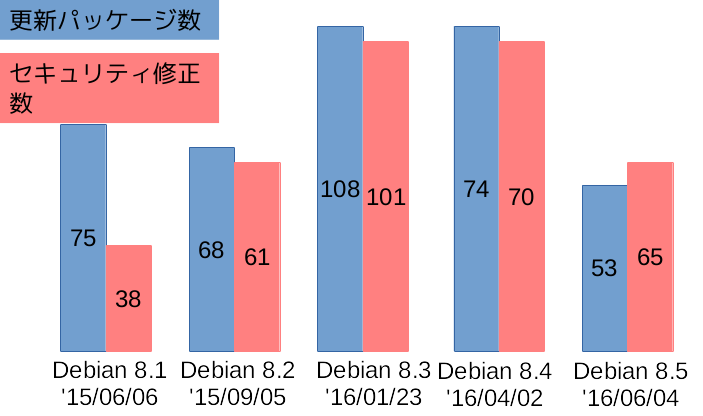
\includegraphics[width=0.6\hsize]{image201606/debian-update.png}
 \end{center}

\item 2016/05/15: ZFS in Debian/contrib

	\begin{itemize}
		\item 注意: Debian に入ったわけではない。main セクションのみが Debian。
		\item DKMS を使うことによってGPLとのCDDLのライセンスコンフリクトを回避。
	\end{itemize}
\end{itemize}
\end{frame}

\begin{frame}{Debian Updates}

\begin{itemize}[<+->]
\item Debug シンボル用パッケージ用新規スイート提供開始 \\ \pause
debhelper 9.20151219以降から、常にデバッグ用シンボルを収めたパッケージ パッケージ名-dbgsym を
生成するようになり、これを提供する stretch 向けサーバが稼働開始した。

\begin{block}{設定するapt-line}
deb http://deb.debian.org/debian-debug stretch-debug main
deb http://deb.debian.org/debian-debug testing-debug main
\end{block}
% http://debug.mirrors.debian.org/debian-debug/

\end{itemize}
\end{frame}

\section{次期リリース Debian 9 について}
\begin{frame}\begin{center}\Huge{次期リリース Debian 9 について}\end{center}\end{frame}

\begin{frame}{次期リリース Debian 9 について}% [containsverbatim]
Debian 9 のコードネームは \pause \\
 \begin{center}
{\Huge stretch} \pause
% \includegraphics[width=0.8\hsize]{image201606/stretch.jpg}
 \end{center}
\end{frame}

\begin{frame}{次期リリース Debian 9 について}% [containsverbatim]

スケジュール

\begin{itemize}
\item 2016年11月5日: transitions freeze
\item 2017年1月5日: "Soft" freeze
\item 2017年2月5日: Full freeze
\end{itemize}

\end{frame}

\begin{frame}{次期リリース Debian 9 について}% [containsverbatim]

サポートアーキテクチャ
\begin{itemize}
\item i386アーキテクチャのサポートCPUをi686以降に変更
\item リリースアーキテクチャ
\begin{itemize}
\item amd64, i386, armel, armhf, arm64, mips, mipsel, powerpc, ppc64el, s390x
\item mips64el が入る可能性
\item armel はBuilddメンテナが少ない。ということで様子見。\\
	aarch32 はarmhf に移行しているため、ユーザも少なくなっているが、まだ人気のあるアーキテクチャ。
\end{itemize}
\end{itemize}

\end{frame}

\begin{frame}{次期リリース Debian 9 について}% [containsverbatim]

サポートアーキテクチャ
 \begin{center}
 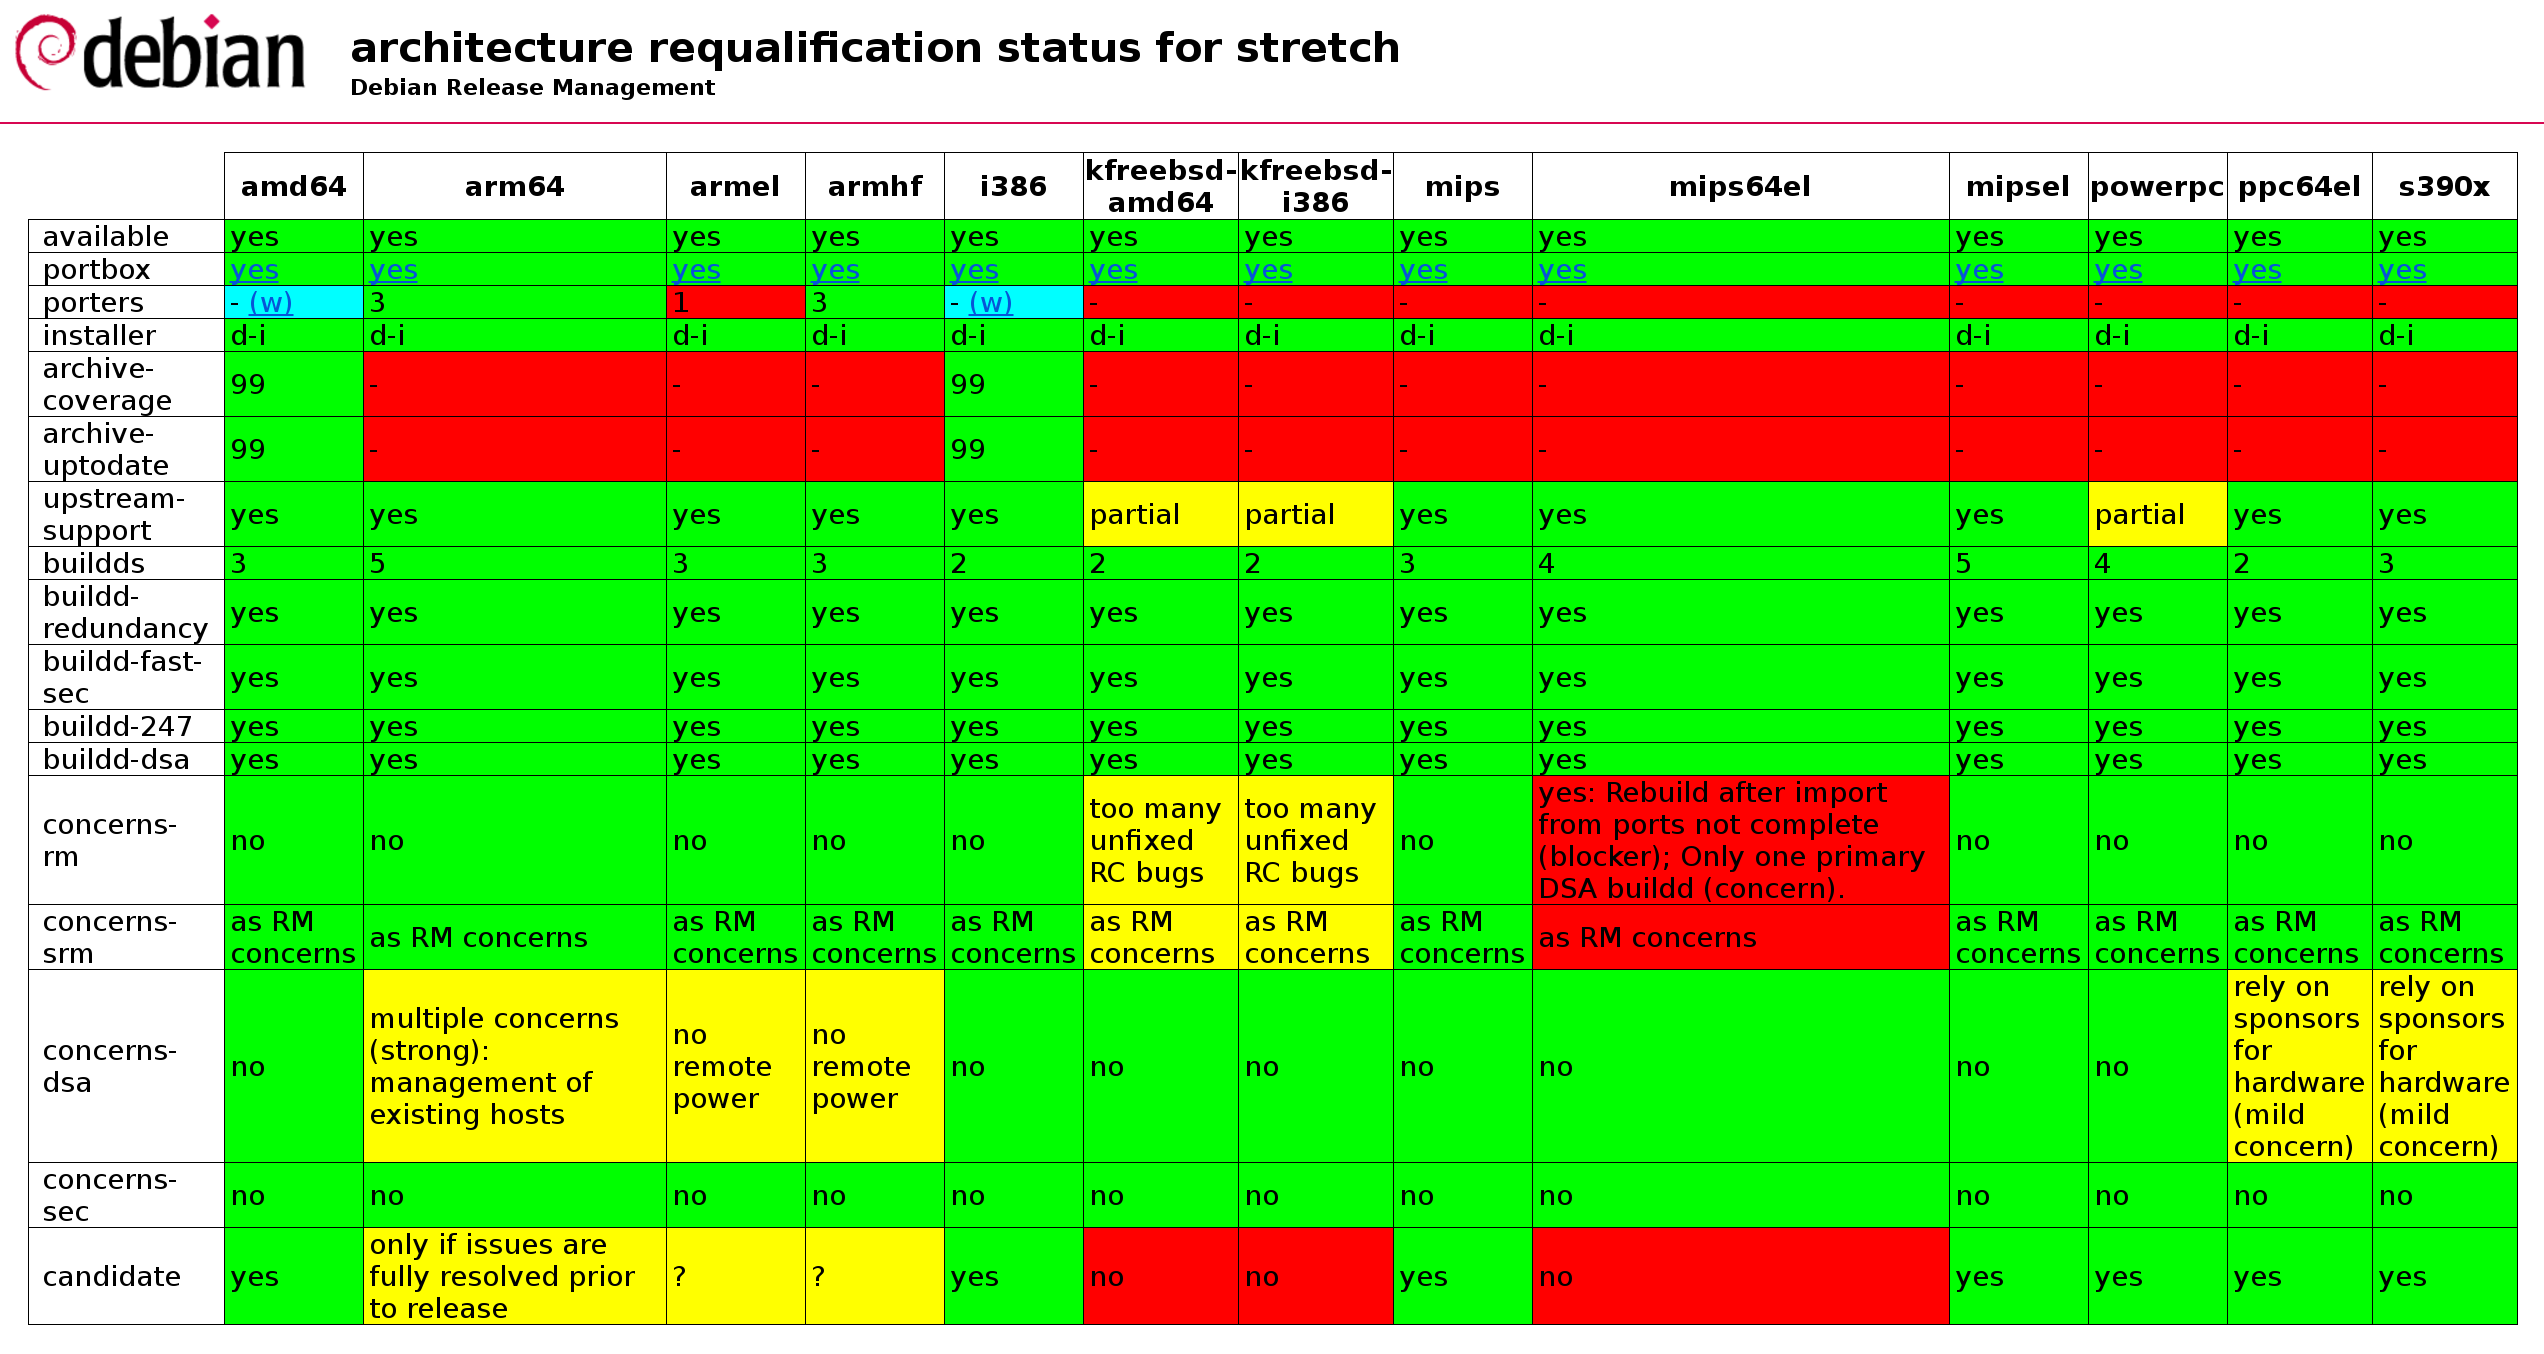
\includegraphics[width=0.8\hsize]{image201606/stretch-arch-requalification.png}
 \end{center}

\end{frame}



\begin{frame}{次期リリース Debian 9 について}% [containsverbatim]

ソフトウェア
\begin{itemize}
\item Linux カーネルは 4.10 をターゲット
\item ツールチェイン(GCC 6, binutils 2.26, glibc 2.22)
\item Perl 5.22 ,Python 2.7/3.6, Ruby 2.3 ,PHP 7.0 ,Go 1.6.1
\item GNOME 3.20, KDE 5.6.4, Xfce 4.12.3, lxde, lxqt 0.10
\item MySQL 5.6.30, MariaDB 10.0.24, PostgreSQL 9.6 beta1
\item etc...
\end{itemize}

アップデートが必要なパッケージがある場合は連絡ください。

\end{frame}

\section{日本語によるDebianの情報}
\begin{frame}\begin{center}\Huge{日本語によるDebianの情報}\end{center}\end{frame}

\begin{frame}{日本語によるDebianの情報}
\begin{itemize}
  \item Debian JP Project \\
      \url{http://www.debian.or.jp}
  \item 東京エリアDebian勉強会\\
      \url{http://tokyodebian.alioth.debian.org}
  \item 関西エリアDebian勉強会 \\
      \url{https://wiki.debian.org/KansaiDebianMeeting}
  \item Twitter \\
      \url{@debian_jp}
  \item G+ コミュニティ \\
      \url{https://plus.google.com/u/0/communities/106942835439686570073}
 
\end{itemize}
\end{frame}

\section{今後のイベント}
\begin{frame}\begin{center}\Huge{今後のイベント}\end{center}\end{frame}

\begin{frame}{今後のイベント}
\begin{itemize}

\item 6月26日 第111回関西Debian勉強会、Debian パッケージング道場
  \begin{itemize}
      \item 京都大学理学部3号館108号室
      \item \url{https://wiki.debian.org/KansaiDebianMeeting/20160626}
  \end{itemize}
\item 6月25日 第140回東京エリアDebian勉強会
  \begin{itemize}
      \item イベント&コミュニティスペース dots.(東京/渋谷)
      \item \url{http://tokyodebian.alioth.debian.org/2016-06.html}
  \end{itemize}

  \item 7月2日 OSC沖縄
  \begin{itemize}
      \item 沖縄コンベンションセンター 会議棟B
      \item \url{http://ospn.jp/osc2016-okinawa}
  \end{itemize}

\item 7月2日〜7月9日 Debconf16
  \begin{itemize}
      \item 南アフリカ共和国 / ケープタウン
      \item \url{https://debconf16.debconf.org/}
  \end{itemize}

\end{itemize}
\end{frame}

\begin{frame}{質問}
\begin{center}
何か質問はありますか?
\end{center}
\end{frame}

\end{document}

;;; Local Variables: ***
;;; outline-regexp: "\\([ 	]*\\\\\\(documentstyle\\|documentclass\\|emtext\\|section\\|begin{frame}\\)\\*?[ 	]*[[{]\\|[]+\\)" ***
;;; End: ***
